% !TeX root = ../main-presentation.tex
\begin{frame}
    \frametitle{What are we going to be talking about?}
    \await
    \centering
    \LARGE
    Digital circuits!

    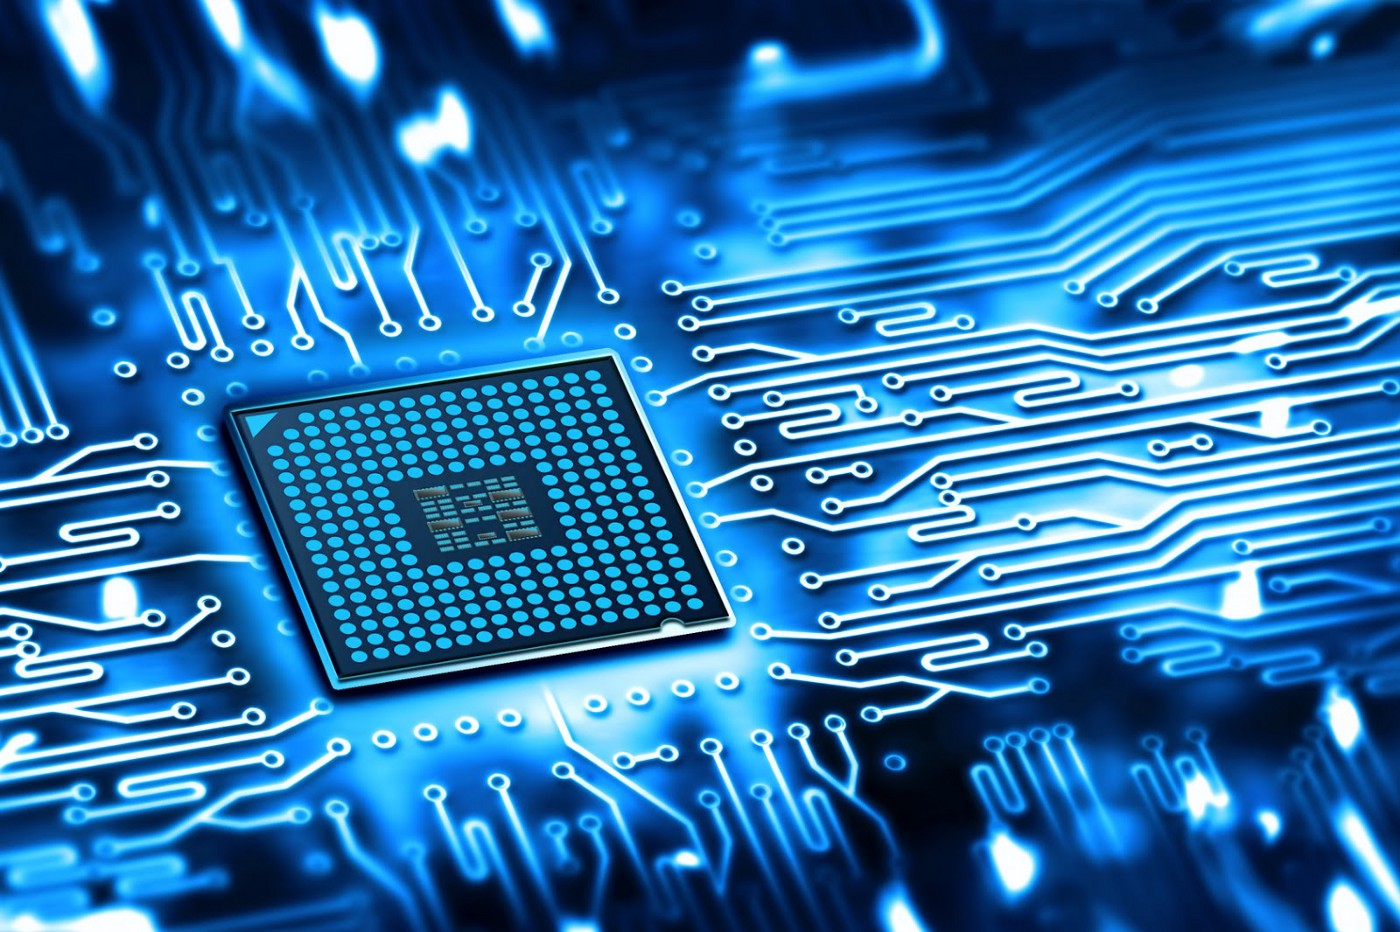
\includegraphics[width=0.6\textwidth]{imgs/circuit}
\end{frame}
\begin{frame}
    \frametitle{What are we going to be talking about?}
    \centering
    \LARGE
    Digital circuits!

    \vspace{1em}
    \normalsize

    \scalebox{2}{\tikzfig{circuits/examples/sr-latch/real-circuit}}
\end{frame}
\begin{frame}
    \frametitle{What are we going to be talking about?}

    \centering
    \Large
    We want a \alert{compositional} theory of digital circuits.

    \vspace{1em}

    \normalsize

    \await
    \dsptikzfig{strings/category/f}[box=f,colour=seq]
    \await
    \quad
    \dsptikzfig{strings/category/f}[box=g,colour=seq]
    \await
    \quad
    \dsptikzfig{strings/category/f-2-2}[box=h,colour=seq]

    \await
    \vspace{1em}

    \dsptikzfig{strings/category/composition}[box1=f,box2=g,colour=seq]
    \quad
    \dsptikzfig{strings/monoidal/tensor}[box1=f,box2=g,colour=seq]
    \quad
    \dsptikzfig{strings/traced/trace-rhs}[box=h,colour=seq]

    \await

    \Large
    \vspace{1em}

    Using \alert{string diagrams} removes \\ much of the bureacracy

    \await

    \normalsize

    (also they look pretty)

\end{frame}

\begin{frame}
    \frametitle{The story so far}

    \centering
    \LARGE

    How did we get here?

    
\includegraphics[width=0.5\textwidth]{imgs/megabus}

\end{frame}

\begin{frame}
    \frametitle{The story so far}

    \centering

    \scalebox{8}{\textbf{2003}}

\end{frame}

\begin{frame}
    \frametitle{The story so far}

    \centering
    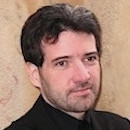
\includegraphics[width=0.3\textwidth]{imgs/lafont}

    \LARGE
    \textbf{Yves Lafont}

    \normalsize
    \emph{`Towards an algebraic theory of Boolean circuits'}

\end{frame}

\begin{frame}
    \frametitle{The story so far}

    \centering

    \scalebox{8}{\textbf{2016}}

\end{frame}

\begin{frame}
    \frametitle{The story so far}

    \centering

    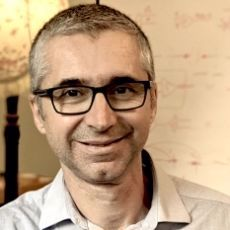
\includegraphics[width=0.25\textwidth]{imgs/ghica}
    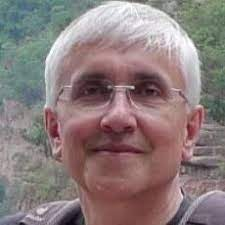
\includegraphics[width=0.25\textwidth]{imgs/achim}
    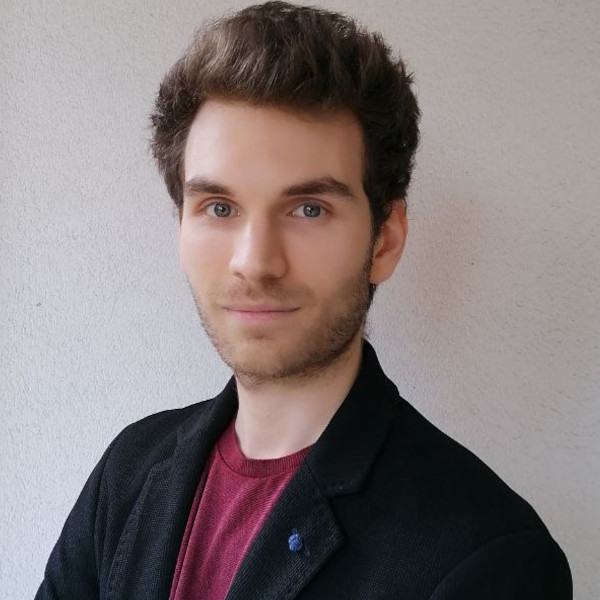
\includegraphics[width=0.25\textwidth]{imgs/lopez}

    \LARGE
    \textbf{Dan Ghica, Achim Jung, Aliaume Lopez}

    \normalsize
    \emph{`Diagrammatic semantics for digital circuits'}


\end{frame}

\begin{frame}
    \frametitle{The story so far}

    \centering

    \scalebox{8}{\textbf{2019}}

\end{frame}

\begin{frame}
    \frametitle{The story so far}

    \centering

    \begin{minipage}{0.45\textwidth}
        \centering

        \phantom{\textbf{David Sprunger}}

        \vspace{0.5em}

        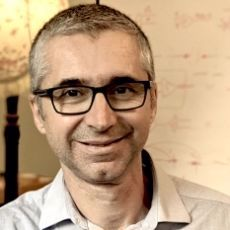
\includegraphics[width=8em]{imgs/ghica}

        \visible<\iftoggle{static}{1}{2-}>{\emph{`Do you know category theory'}}

        \visible<\iftoggle{static}{1}{4-}>{\emph{`Do you want to do circuits stuff'}}
    \end{minipage}
    \begin{minipage}{0.25\textwidth}
        \centering

        \phantom{\textbf{David Sprunger}}

        \vspace{0.5em}

        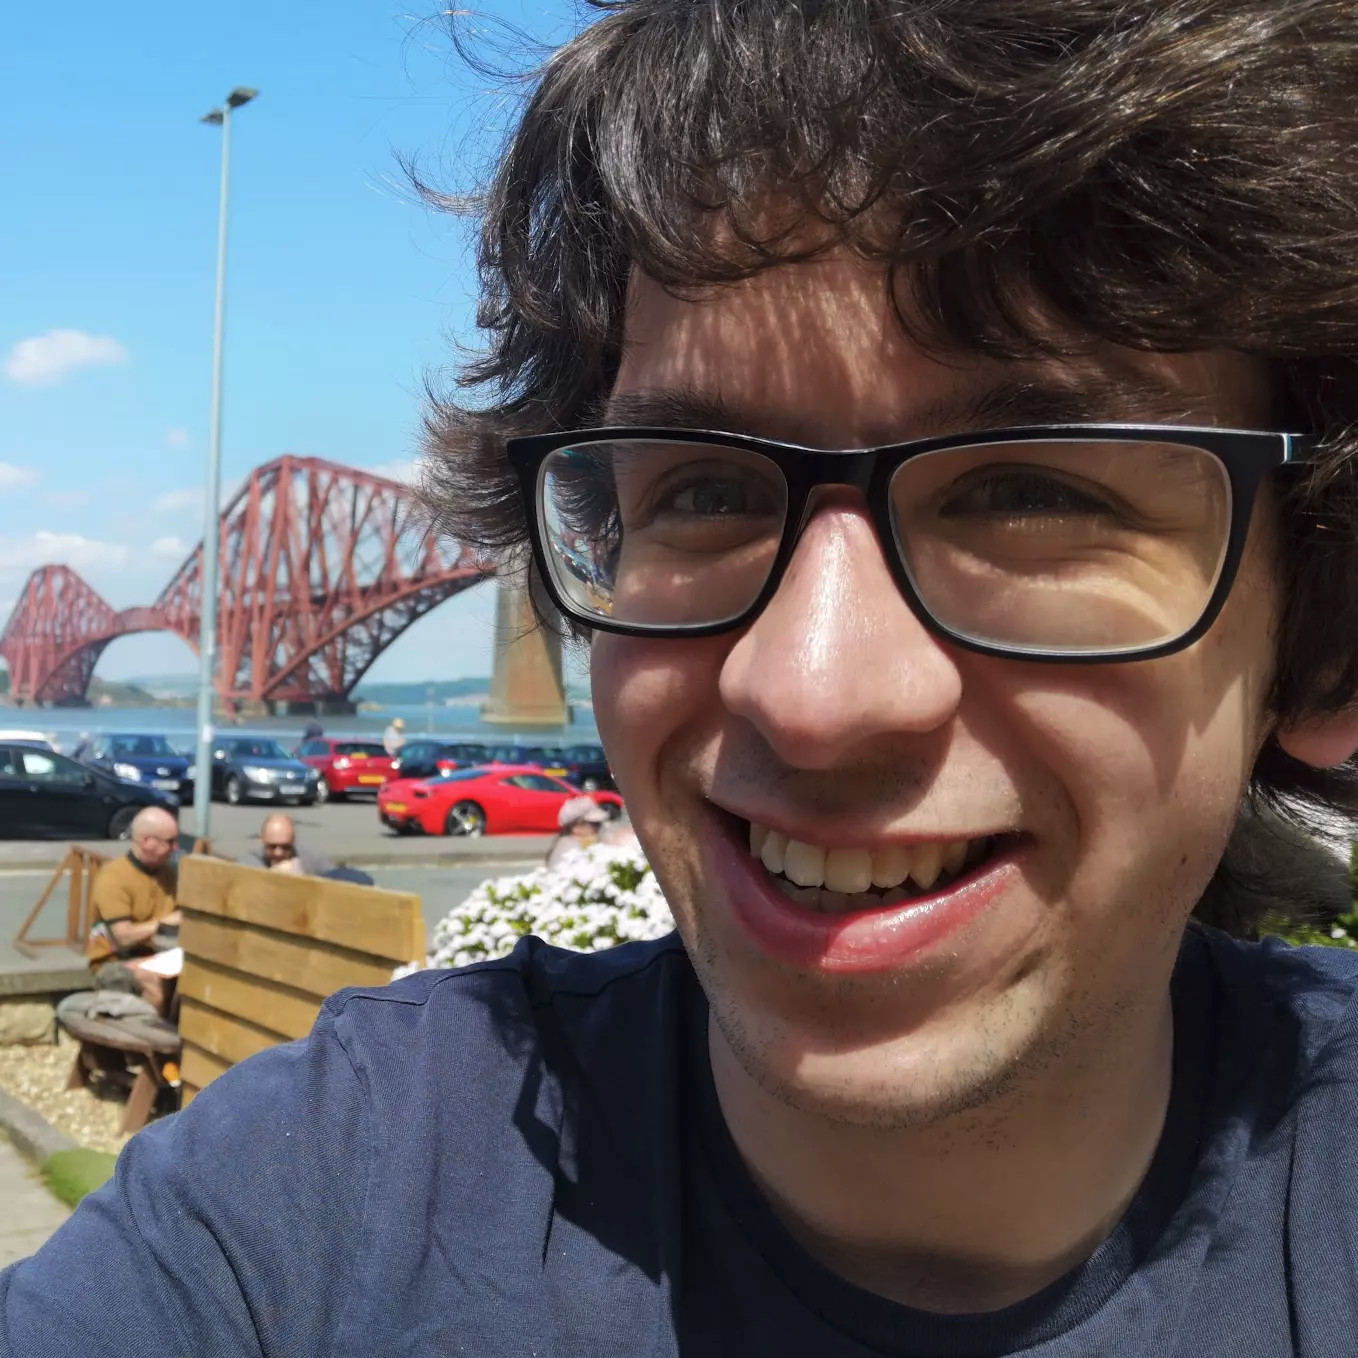
\includegraphics[width=8em]{imgs/kaye}%

        \visible<\iftoggle{static}{1}{3-}>{\emph{`No'}}

        \visible<\iftoggle{static}{1}{5-}>{\emph{`Okay'}}
    \end{minipage}
    \visible<\iftoggle{static}{1}{6-}>{%
        \begin{minipage}{0.25\textwidth}
            \centering

            \textbf{David Sprunger}

            \vspace{0.5em}

            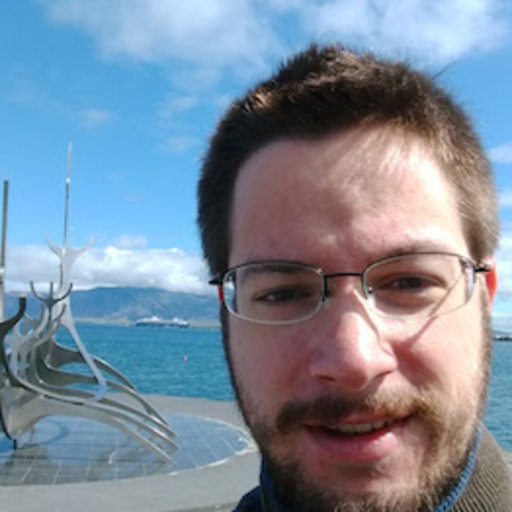
\includegraphics[width=8em]{imgs/sprunger}

            \phantom{hello}

            \emph{`I will help too'}
        \end{minipage}%
    }
\end{frame}